%!TEX TS-program = xelatex
%!TEX encoding = UTF-8 Unicode

\documentclass{../Dissertate}

\begin{document}

\doublespacing

\setcounter{chapter}{2} % This chapter minus 1
\chapter{Perceptual Similarity vs. Conceptual Knowledge in Induction}

\section{Introduction}

In Chapter 3, we saw that 
induction can be driven by more than one kind of information,
as perceptual similarity and conceptual knowledge
came into conflict during reasoning.
\citet{Bright2014a}, in their hybrid theory,
proposed a more subtle distinction in inductive reasoning,
between associative and structured knowledge.
While a number of results show that both kinds of knowledge
can drive inductive reasoning, however,
less is known about how these kinds of knowledge interact.
This is the question I seek to answer in this chapter.

As \citet{Bright2014a} note,
theories of induction can be classed in two ways.
Some theories propose that induction is based on structured knowledge:
the world is organised into coherent categories,
and specific knowledge about these categories,
and the often complex relationships between them,
is used as the basis for inference.
One such theory is \citegap{Osherson1990}{'s} similarity coverage model,
that describes inferences about species of animal
with reference to the taxonomic relationships between them.
More recent accounts have generalised this idea,
casting induction as a process of Bayesian inference
\citep{Griffiths2009,Griffiths2005,Heit1998,Kemp2009}.
At the core of these accounts is the notion that
in category-based induction,
we attempt to use the information given in the premises
(i.e. ``Carrots have disease X'')
to update our beliefs about the distribution of this property
across all categories.
To do so, we must be able to express how various categories are related:
the probability that rabbits have a given disease, given that carrots have it,
depends on the means by which diseases can be transmitted between various species,
in this case, through ecological interactions, such as a food chain.
Similarly, biological properties, such as genes,
are most strongly projected according to 
the distance between species in the taxonomic tree \citep{Heit1998,Osherson1990},
while if we know that certain artefacts are found in one city,
geographical distance is used to decide which other cities are likely to
house them \citep{Kemp2009}.

On the other hand,
a number of theories of inductive inference,
and category-based induction in particular,
rely on simpler, \emph{associative} forms of knowledge.
Similarity, including visual similarity,
discussed in Chapter 3, is one such form of knowledge;
things that are similar
\citep[share many properties, or features, that we know of; see][]{Medin1993}
are likely to also share novel properties.
For instance, on learning about two animals, both of which
live underwater, have scales, and breathe through gills,
we do not need to know what a ``fish'' is
to predict that if one lays eggs, the other likely does as well.
Of course, as discussed in Chapter 3, similarity comes in many forms,
and \citet{Fisher2015} make a useful distinction between
perceptual and representational (i.e. knowledge-based) similarity.
Perceptual similarity is most often proposed
as the basis of induction in children
\citep[][see also Chapter 3]{Sloutsky2010,Sloutsky2008,Sloutsky2007}.
A number of theories of induction in adults,
however, are based on the overlap of features
in our mental representations \citep{Rogers2004,Rogers2008,Sloman1993}
or perceptual input \citep{Sloutsky2008,Sloutsky2004}.
Other associative accounts of induction,
including of inductive generalisation during learning, are based on
what is variously referred to as contiguity, co-occurrence, or thematic relations:
things that are often seen together are more likely 
to share properties than things that are not
\citep{Kruschke1992,Rumelhart1986,Rescorla1972}.

% Also cited:
% Colunga & Smith, 2005;
% French, Mareschal, Mermillod, & Quinn, 2004; Jones & Smith, 2002; Sloutsky, Kloos, &
% Fisher, 2007).
% Smith and DeCoster (2000)

\citet{Bright2014a} argue that neither
structured nor associative accounts of induction alone are complete.
As noted by \citet{Murphy1985},
associative accounts of categorisation and induction
fail to capture some of the flexibility and complexity seen in human reasoning.
In particular, participants have been shown to be
sensitive to property effects when reasoning inductively:
the strength of an argument is dependent
on the kind of property projected
\citep{Heit1994,Shafto2007,Shafto2005}.
Therefore, transmittable properties such as infectious diseases
are thought to be shared by animals that are related ecologically,
such as predators and prey in a food chain,
whereas biological properties such as genes are shared 
only by animals that are close together in their taxonomic tree.
It is difficult to account for such flexibility in a purely associative account
\citep[but see work by][]{Sloutsky2008,Rogers2004}.
Structured models such as the Bayesian accounts discussed above \citep[i.e.][]{Kemp2009},
in contrast, draw on different knowledge structures for different inferences,
and so can capture this flexibility in human reasoning.

At the same time, it seems unlikely that 
structured knowledge alone drives inductive reasoning.
Induction is an ubiquitous phenomena, encompassing any inference that goes
``beyond the information given'' \citep{Bruner1973}.
This ranges from simple perceptual inferences,
to the development and postulation of scientific theories
\citep[see][for a taxonomy of inductive inferences]{Kemp2014}.
Furthermore, inductive reasoning is not exclusive to human adults:
similar inferences, although in simpler domains,
must be made both by children, and throughout the animal kingdom.
Associative theories of induction provide accounts that
make more reasonable claims about the cognitive abilities
required to reason inductively.
Indeed, in the spirit of \citet{Simon1956},
associative processes may \emph{satisfice},
often yielding the same inferences as structured accounts,
but with considerably less effort.

Faced with this dichotomy between associative and structured knowledge in induction,
\citet{Bright2014a} proposed a theory that combines both forms of knowledge.
This \emph{hybrid} theory claims
that both kinds of knowledge are drawn upon during reasoning,
with a key distinction between the two being their processing characteristics.
By this account, associative knowledge can be retrieved quickly and easily,
while structured knowledge is slower to retrieve,
and places greater demands on working memory to utilise.

Evidence for this hybrid theory
comes from experiments that manipulate 
the processing conditions under which participants reason.
This research is discussed in more detail in Chapter 1, but to recapitulate,
participants' inferences (their choices, or ratings of argument strength)
are predicted by measures of associative knowledge under all circumstances.
Furthermore, under favourable conditions only
(i.e. in the absence of time pressure, or cognitive load),
inferences are additionally predicted by
appropriate measures of structured knowledge,
such as whether participants believed two species
belonged to the same taxonomic group
when reasoning about biological properties.

Of particular relevance to this thesis, which focuses on \emph{conflict} in reasoning,
\citeauthor{Bright} (\citeyear{Bright}, see also \citealp[Chapter 5]{Crisp-Bright2010})
report a version of the inductive triad task \citep{Gelman1986}
that places associative and structured knowledge directly in conflict.
In the trial shown in Figure~\ref{fig:crisp_screenshot}, for example,
participants were told a biological property of carrots (they have ``C5s cells''),
and chose between generalising this property to rabbits, or to bamboo.
Carrots and rabbits are strongly associated,
and so a participant relying on associative knowledge
would project a property from carrots to rabbits.
This is despite the fact that the link between the species is a food chain,
and so doesn't provide a means for them to share a biological property.
Carrots and bamboo, on the other hand, are both plants,
and so are more likely to share such a property.
The associative link between the two species, however,
is substantially weaker, and so projecting the property to bamboo
requires that one inhibits the associative knowledge linking carrots and rabbits
before one can draw on the structured link between carrots and bamboo instead.
Consistent with the hybrid theory,
participants were less likely to select the
taxonomically-related response option
over a strongly associated foil in this task
when under heavy cognitive load,
or if they had poor semantic inhibitory control
\citep[a measure of their ability to inhibit
  task-irrelevant semantic information;][]{Markovits2004,Burgess1996a}.
Like most studies that analyse only participants' ultimate responses, however,
while these results do reveal what information drove participants' final choices,
we are limited in what conclusions we can draw about
how different processes interact during this task.
To address this shortcoming, in this chapter I present
a mouse tracking extension of the \citet{Bright} triad task.

\begin{figure}[ht]
  \centering
  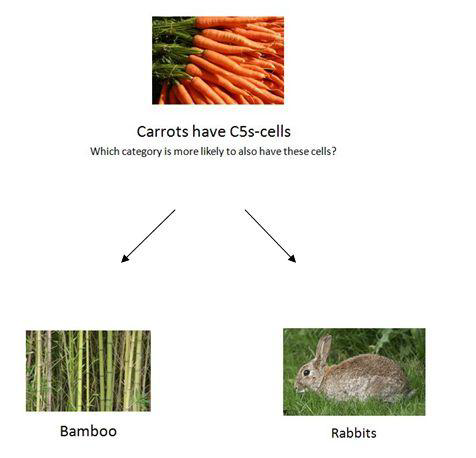
\includegraphics[width=\figurewidth]{imgs/crisp_screenshot.png}
  \caption[A conflict trial from \citet{Bright}.]{
    A conflict trial from \citet{Bright}.
    Participants learn that carrots posses the given biological property,
    and asked which of the other two species, bamboo or rabbits,
    are likely to share this property.
    \label{fig:crisp_screenshot} }
\end{figure}


How might associative and structured knowledge interact during this task?
Again, I propose two possibilities.
First, it may be that people selectively draw on associative knowledge
\emph{or} structured knowledge for a given inference.
In this case, we would expect to find
little evidence of actual conflict during reasoning,
as both kinds of knowledge would not compete during a single trial.
This would lead to cursor trajectories where
participants move directly towards one or other option, and then select it,
rather than changing direction mid-flight.
The second possibility is that
associative knowledge may be activated early in reasoning,
but be later overridden, at least some of the time,
by slowly-retrieved, more cognitively demanding structured knowledge.
In this case, participants would be conflicted
when they do override, or at least attempt to override,
their association-driven response.
Cursor trajectories in this case should largely be
initially drawn to the foil species
when it is cued by associative knowledge,
but also likely to override this initial movement
and select the correct species instead
at least some of the time.







\section{Experiment 1}

In Experiment 1, participants completed
a mouse tracking version of \citegap{Gelman1986}{'s} triad task,
with natural categories.
In the original version of this task, children had to choose
between generalising a property from a base species
to another conceptually-related species,
or to an unrelated but perceptually similar one.
This experiment is, to my knowledge,
the first to include a control condition,
in which both perceptual and conceptual information cue the same response.
Using this experimental manipulation, it is possible to
explore the role these perceptual cues play in reasoning.
Additionally, by recording participants' mouse cursor movements,
the experiment provides a window into processes during reasoning,
rather than just the final inferences participants make.



\subsection{Method}

\subsubsection{Participants}

Fifty nine undergraduate students took part in exchange for course credit.

\subsubsection{Stimuli \& Procedure}

At  the start of the experiment,
participants were presented with a framing story,
based on those used by \citet{Sloutsky2007} and \citet{Gelman2013c}.
This introduced a boy, Mark, who had moved to a country called Elbee,
where his teacher was teaching him
about the plants and animals found there.
They were instructed that they would be told
some of the facts that Mark's teacher had told him,
and shown pictures of three animals.
They were also instructed that their task was to decide,
given a fact about one species,
which of the two other species
this fact was likely to be true for.
This was illustrated using an example.

Participants then completed ten induction trials, in random order.
Induction stimuli were similar to those used by \citet{Gelman1986},
but were created for the current experiment.
They consisted of ten sets of species of plants and animals.
The full set of stimuli used can be found in Appendix~\ref{appendix:exp1_stimuli}.
Each set was made up of a \emph{base} species,
a \emph{correct response} species belonging to
the same super-ordinate category as the base,
and two \emph{foil} species, belonging to a different category:
one that was intended to be
perceptually similar to the base, and one that was not.
Each species was represented in the experiment
by a colour photograph (see Figure~\ref{fig:exp1-screenshot1},
and Appendix~\ref{appendix:exp1_stimuli}).
For each participant, five stimuli sets were randomly chosen as
conflict trials, and presented with the foil
that was perceptually similar to the base.
The remaining sets were designated control trials
and presented with the foil dissimilar to the base.

On each trial, the base was presented
in the centre of the screen,
with a property of that species shown above the image.
Blank genetic properties were used, of the form
``This one has gene 4ew. What else do you think has gene 4ew?''.
After clicking a button marked ``NEXT'' in the bottom centre of the screen,
images of the two possible response species
appeared in the top left and right corners,
with their positions randomised on each trial
(Figure~\ref{fig:exp1-screenshot1}).
Participants responded by clicking on one or other image,
and the position of the mouse cursor was recorded as they did so.

\begin{figure}[pt]
  \centering
  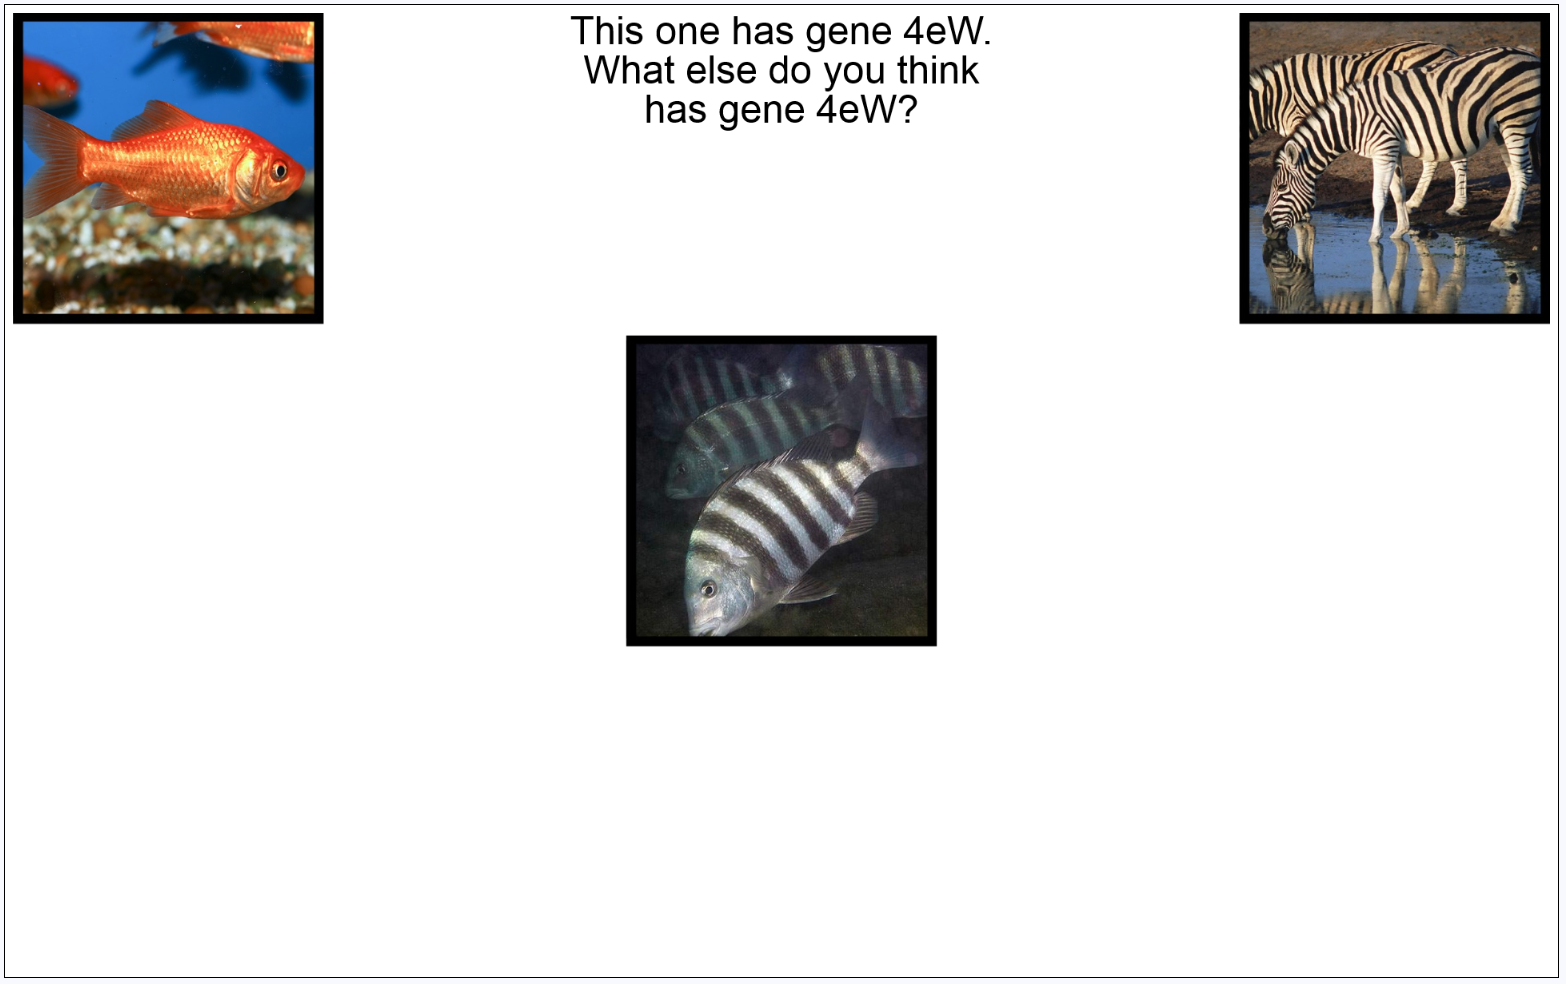
\includegraphics[width=.8\textwidth]{imgs/natural_conflict.png}
  \caption[Screen shot of conflict trial from Experiment 1.]{
    Screen shot of conflict trial from Experiment 1.
    The base image, a striped fish, belongs to the same category as the
    correct response option, the goldfish shown in the top left,
    but is perceptually similar to the foil option,
    the zebra in the top right.}
  \label{fig:exp1-screenshot1}
\end{figure}

\begin{figure}[pb]
  \centering
  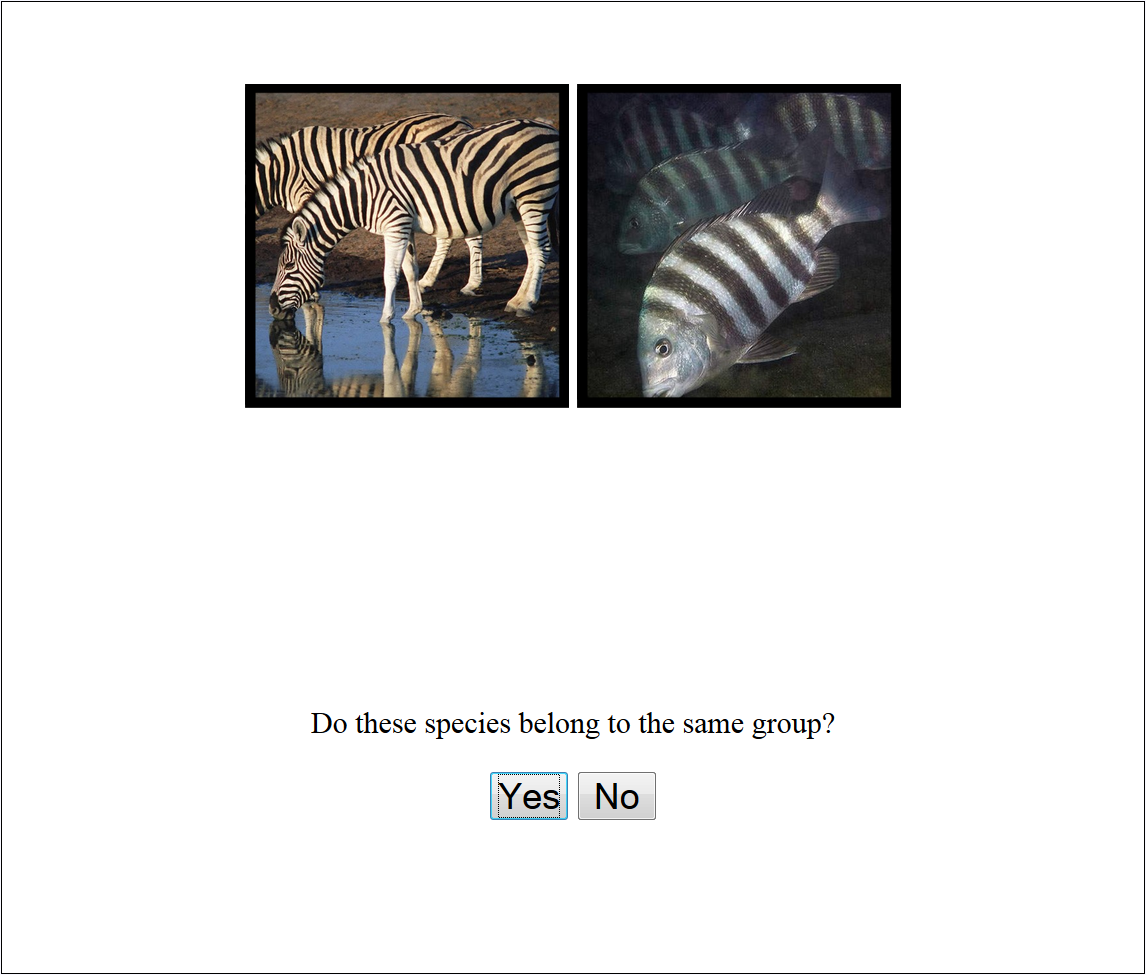
\includegraphics[width=.7\textwidth]{imgs/exp1_posttest.png}
  \caption{Screen shot from the post-test check, Experiment 1.
    \label{fig:exp1-screenshot2}}
\end{figure}


After the reasoning trials, participants completed a post-test check.
This was to ensure that participants possessed the appropriate
structured knowledge about the relationships between
the species used.
Each base species was presented twice,
once alongside its corresponding correct response,
which belonged to the same biological category,
and once alongside its perceptually similar foil,
which did not.
The left-right positioning of these images
was randomised for each trial.
Participants were instructed to indicate
if each pair of species belonged to the same biological group.
% (Figure~\ref{fig:exp1-screenshot2})
The order of presentation of the post-test stimuli was totally randomised.


\section{Results}

\subsection{By-trial analyses}

After excluding data from 3 participants 
who did not complete the experiment within the 15 minutes allocated, 
and 7 trials with response times greater than 100 seconds (.6\% of the total), 
participants selected the correct option on 79.5\% of non-conflict problems.
On the conflict problems, the correct option was chosen 36\% of the time,
the heuristic option 58\%, and one of the foils 6\% of the time.

In the first stage of the analysis, 
I calculate a number of summary statistics for each trial, 
and compare these between problem types, and between responses. 
The measures were response time, 
the distance travelled by the mouse cursor
(scaled so that a straight line from the start point
 to the response corresponds to 1 unit),
the number of times the cursor was moved during a trial
(with movements defined as windows of 100 msec or more in motion, 
separated by 100 msec or more not moving), 
the closest proximity achieved between 
the cursor and the non-chosen option
(closest proximity to the heuristic response option 
on trials where the correct option was chosen, and vice versa). 
These measures were compared using linear mixed models, 
with crossed random intercepts for each participant, 
and each problem \citep{Baayen2008}.
Response latencies, and the distance travelled by the mouse cursor
were log-transformed to normalise their distributions, 
and a generalised mixed model with a Poisson link was used
to model the number of movements. 

Consistent with a dual process interpretation, 
whereby heuristic responses are generated by Type 1 processes,
and correct responses under conflict by Type 2 processes,
for conflict problems there was greater evidence of conflict
across all measures when participants gave the correct response (N = 181) 
than the heuristic one (N = 297).
The average time to respond was 27.3 seconds (SD = 16.3) for correct responses, 
and 21.0 seconds (SD = 13.4) for heuristic responses
($e^{\beta}$ = 114\%, CI = [102\%, 129\%],
t(470.8) = 2.349, p = .0192).
The mouse cursor travelled a greater distance 
before selecting a correct option (6.11 times the minimum needed distance, SD = 5.6) 
than an heuristic option (5.66 times, SD = 4.74;
$e^{\beta}$ = 116\%, CI = [102\%, 133\%],
t(298.4) = 2.267, p = .0241). 
There were also more cursor movements on
trials in which the correct response was given (5.4, SD = 4.8) 
than when the heuristic response was given (4.9, SD = 4.5; 
$e^{\beta}$ = 1.15, CI = [1.02, 1.29],
z = 2.337, p = .0195).
Finally, the minimum distance between 
the cursor and the heuristic option on trials in which the correct option was chosen 
was on average 49\% of the display width (SD = 24\%),
significantly less than the minimum distance between
the cursor and the correct option 
on trials in which the intuitive option was chosen (55.5\%, SD = 18\%,
$e^{\beta}$ = 0.92, CI = [0.89, 0.96],
t(72.1) = 4.119, p < .0001).

Most tests of the intuitive logic model compare
correct responses on no-conflict problems with
heuristic responses on conflict problems, 
on the basis that heuristic, Type 1 processes should cue both kinds of response, 
but the chosen response conflicts with normative principles on conflict problems only. 
Evidence for the intuitive logic model 
therefore comes from results which indicate 
greater conflict for heuristic responses to conflict problems (N = 404). 
However, there was no such reduction in conflict for no-conflict problems
on any of the applicable measures:
response time (23.1 seconds, SD = 15.3; t(14.3) = 0.222, p > .8),
distance travelled (5.6, SD = 5.0; t(15.0) = 0.359, p > .7) 
and number of movements per trial (5.2, SD = 4.6; z = 0.064, p > .95).

Following previous intuitive logic studies
\citep[e.g.][see also \citealp{Pennycook2015}]{DeNeys2011b,Mevel2014},
I also calculated the number of heuristic responses given
by each participant on conflict problems, 
and categorised each participant as either
``majority heuristic'' (3 or 4 heuristic responses out of four, 53 participants)
or ``minority heuristic'' (0 to 2 heuristic responses, 75 participants). 
I entered this measure as a participant-level predictor in the models, 
but found that it was not involved with any interactions in the analyses above
(t's < .9, p's > .4). 
I also repeated this analyses for the most (4 heuristic responses) 
and least (one heuristic response) biased reasoners only, 
again finding so significant interactions (t's < 1.1, p's > .25).
Therefore, these analyses revealed no evidence for logical intuitions
in either biased or unbiased participants.



\subsection{Discussion}

This experiment placed perceptual similarity
and conceptual knowledge in conflict
in an inductive reasoning task.
My first goal in doing so was to test the prediction,
based on \citegap{Bright2014a}{'s} hybrid theory,
that adults' inferences would be influenced by perceptual cues,
as well as conceptual knowledge.
This prediction was confirmed by participants' responses:
when conceptual knowledge did not conflict with perceptual similarity,
participants selected the conceptually-cued response on almost every trial.
When the foil species looked similar to the base, however,
participants chose the foil 40\% of the time.
Additionally, this effect was found for the vast majority of participants,
and so is not the result of a few participants who are
inappropriately swayed by these visual cues.
When participants did give the correct response,
it appears that they experienced conflict
when perceptual cues supported the foil response,
taking significantly longer to respond,
and being more likely to initially move towards
the perceptually-cued foil option.

The mouse tracking paradigm makes it possible
to go beyond this finding, however,
and work towards a description of
how these two sources of information interacted during reasoning.
In Chapter 1, I raised two possibilities:
participants may either selectively use one or other cue,
or they may use perceptual cues by default,
but reject them in favour of conceptual knowledge
when they realise those cues to be inappropriate.
Consistent with both possibilities,
on control trials, where the base and the foil did not look alike,
participants initially moved towards the foil 21\% of the time.
On conflict trials, where they did look alike,
participants initially moved towards the foil 57\% of the time.
Furthermore, these movements %towards the foil under conflict
were initiated faster than movements towards the correct option in the same condition,
suggesting either
that conceptual knowledge takes longer to utilise than perceptual cues,
or that perceptual cues must be inhibited on these trials.

These two possibilities can be distinguished by looking to
what participants do when they have initially moved towards
a perceptually-cued foil.
In this situation, participants changed direction on 45\% of trials
to select the correct option instead.
By comparison, participants who initially moved towards the correct option under conflict
only changed direction to select the foil on 19\% of trials.
Therefore, it appears that, at least some of the time,
reasoning on the basis of conceptual knowledge required
the inhibition of the response based perceptual cues.
Together, these results suggest that perceptual cues
are used by default on this task.
By this view,  participants can either
initiate an early movement, driven by these cues (57\% of the time),
and subsequently either inhibit this response (45\% of the time),
or follow through with it and select the foil species.
Alternatively they can override these cues
before they move the cursor (43\% of the time),
and move directly towards the correct option.

Analysis of the time course data also appears to support this interpretation.
In Figure~\ref{fig:exp1_side_timecourse} we see that
on conflict trials, participants were initially (300 to 1,340 msec)
more likely to be on the foil side of the screen than the correct side.
By 1,940 msec, however, this trend had reversed,
and participants were instead more likely to be on the side of the correct option.

An interesting question, which this experiment does not answer,
is what factors dictate whether or not participants
moving towards the foil ultimately select this option,
or instead override this initial movement and select the correct species.
  %% In particular, a lot of recent Thompson/Pennycook work
  %% has looked at determinants of reflection from a DI perspective.
  %% Their account talks about metacognition, and Feeling of Rightness,
  %% in contrast to De Ney's intuitive conflict detection idea.
  %% For now, I'll just cite that work here, on the basis that
  %% the next draft of Ch1 will review it.}
This issue has come under increased scrutiny lately in the dual process literature
\citep[see, for instance,][]{Thompson2014a,Thompson2011,DeNeys2012,Pennycook2015},
where the focus has been on whether participants
reflect on their intuitive responses.
In the induction literature,
\citet{Gelman2013c} report a series of experiments with children
using the triad task.
They show that children are more likely to
use conceptual knowledge, rather than perceptual similarity,
when the conceptual categories used differed at a high, ontological level,
(animals versus robots),
than when they differed at a lower level (kinds of dogs, or creatures categorised
according to their ratio of fingers to chest buttons,
as used by \citealp{Sloutsky2007}).
They also demonstrated that children are more reliant
on conceptual knowledge when the properties under consideration
are meaningfully related to the different categories,
for instance animals being warm blooded, or robots containing batteries.
Both of these effects make sense from a normative perspective:
categories which are more conceptually distinct
provide a better basis for induction \citep{Rosch1976},
and certain kinds of category are conducive to
the projection of certain kinds of property,
for instance biological properties within biological categories
\citep{Heit1994,Shipley1993,Shafto2007}.
We would expect these same factors to influence adults' inferences.
However, it is not clear at what point in the reasoning process
such variables are important:
they may prompt reasoners to attempt
to draw on conceptual knowledge in the first place,
or they may cause them to be more likely to inhibit
their initial inappropriate perceptually-driven responses.

In Experiment 2, I presented participants with a version of this task
using artificial categories, specifically, a kind of animal, and a kind of robot.
I also manipulated, between participants,
the nature of the kind of properties being considered,
in order to investigate the effect this has on participants' reasoning.


\section{Experiment 4}

In Experiment 4, I attempted to replicate the findings of Experiment 3,
but without the need to discard data from
trials for which participants lacked appropriate taxonomic knowledge.
Beyond this, I wished to explore
how each participants' own beliefs about the strength of association
between various species interacted with structured knowledge during reasoning.
Therefore, in this experiment, I asked participants to rate
the association between each base species
and every response species it was paired with for the reasoning trials.
This improves on the method used in the previous study in two ways.
First, while \citet[Chapter 2]{Crisp-Bright2010} collected
ratings of the association between the base species,
the correct response species, and the strongly associated foils used in the previous experiment,
she did not collect ratings for the associations between the bases
and the foil species assumed to be weakly associated.
Second, \citet{Crisp-Bright2010} collected
association ratings from one set of participants,
and reasoning data from another.
Therefore, it was the average association rating between species
that she used as a predictor in here analyses.
Here, on the other hand, I collected each participants'
own idiosyncratic ratings of the associations between the species,
allowing a more fine-grained analysis of
how such associative knowledge influences reasoning.


\subsection{Method}

\subsubsection{Participants}

Forty four undergraduate students completed the experiment
in exchange for course credit, in a laboratory.
The experiment was programmed using the OpenSesame experiment builder
(see Chapter 2).

\subsubsection{Stimuli}

In the experimental trials, participants were asked about
biological properties, specifically cells.
Nine new stimulus sets were generated for the experimental trials,
intended to be more familiar to participants
than those used in Experiment 3.
Each new set had three foil species,
one intended to be weakly, one moderately,
and one strongly associated with the base.
Each set was presented three times, once with each foil species.
Stimuli were selected according to a number of partial pretests,
in which participants rated the strength of association between species
using the procedure from \citet[][Chapter 2]{Crisp-Bright2010}, described above.
The full set of stimuli can be found in Appendix~\ref{appendix:exp4_stimuli}.

For the filler trials, where participants were asked about diseases,
an additional fourteen stimulus sets were generated,
each containing a base species,
a correct response species likely to share a disease with the base,
and three different foil responses, one for each time the set was presented.
One possible concern about the design of Experiment 3
is that the species designated as the correct response
for each experimental stimulus set
was the correct response on every trial it featured in.
Therefore, the fourteen correct response species from the experimental trials here
were used as foil species (that is, the species that
were unlikely to share a disease with the base species)
on three different filler trials.
This meant that these species were the correct response option
in the three experimental trials in which they featured,
but also the incorrect response option in three filler trials.
The properties to be reasoned about ---
genes on the experimental trials,
and diseases on filler trials~---
were unchanged from Experiment 3.

To ensure that participants did not complete
experimental trials with the same base species in close succession,
the order of trials was randomised with constraints for each participant.
First, the experimental trials were randomly divided
into three blocks of nine trials,
with each block containing
three weak, three moderate, and three strong foils,
and one trial from each stimulus set in each.
Nine of the twenty-seven filler trials were then added to each block.
Finally, the order of trials within each block was randomised repeatedly,
until at least 5 trials separated repetitions of each base species.

\subsubsection{Procedure}

There were minimal changes to the reasoning trials from Experiment 3.
However, this experiment was conducted using the OpenSesame platform,
which allowed greater experimental control over the mouse cursor.
Therefore, instead of requiring participants
not to move the cursor during the fixation period,
the cursor's position was automatically reset
to the centre of the START button after the fixation.

After the reasoning trials, participants again completed a post-test check.
In the first part of the post-test, participants rated the strength of association
of the thirty-six base-response species pairs from the experimental trials.
These consisted of the nine base species,
each of which was paired with its correct response species
and its three foil species.
For this section, participants were presented with the following instructions,
taken directly from  \citet[][Chapter 2, p. 60]{Crisp-Bright2010}:

\begin{quote}
  [...] Please think about all kinds of possible associations, such as causal,
  functional, categorical, etcetera. Please do not think in detail about
  the mechanism by which they are related, just give your intuitive
  response. For example, if you believe that ladybirds and butterflies
  are strongly associated please give a rating closer to 9. In contrast,
  if you think cars and ladybirds are unrelated, please give a rating
  closer to 1. Please give the answer that first comes to mind, as fast
  as possible.  
\end{quote}

On each rating trial, the labelled images of each species
were shown side by side, with their positions randomised.
Participants gave their ratings by clicking on buttons
labelled 1 to 9 below the images,
with 1 subtitled ``Not associated at all'',
and 9 subtitled ``Very strongly associated''.

The second part of the post-test checked participants' structured knowledge.
Participants were presented with pairs of species,
in the same format as the association rating trials,
and gave yes or no responses by clicking the marked buttons.
There were three blocks in this part of the post-test,
and the order of trials within each block was randomised.
First, for each of the nine experimental stimulus sets,
the base species and the correct response species
belonged to the same taxonomic group.
These nine pairs of species were presented along with
an additional nine pairs that did not belong to the same group.
Participants were asked in each case if the pair shown
belonged to the same \emph{biological group}, and told
``Biological groups are the main branches
when you think about the `family tree' of the natural world'',
and that the biological groups in the experiment were
mammals, fish, reptiles, birds, and plants.

Second, for five of the experimental stimulus sets,
the base species was related to the moderately and strongly associated foils
via a food chain relationship --- one species eats the other.
These ten base-foil pairs were presented along with
ten other species pairs not related in this way.
Participants were asked if each pair shown belonged to the same \emph{food chain},
and told ``Species belong to the same food chain if one is eaten by the other
(predators and prey for animals, or a plant which is eaten by an animal)''.

Finally, for the remaining four experimental stimulus sets,
the base species was related to the moderate and strong foils
in that they shared an ecological habitat.%
\footnote{
  This was not technically true for penguins and arctic wolves,
  and penguins and polar bears, as these species live in
  opposite polar regions, but the post-test data showed that
  participants do not realise this.
}
These eight base-foil pairs were presented along with
the eight other pairs that did not share a habitat,
and participants were asked if thee pair shown ``live in the same kind of habitat''.




\subsection{Time Course Analyses}

\begin{figure}[ht]
  \centering
  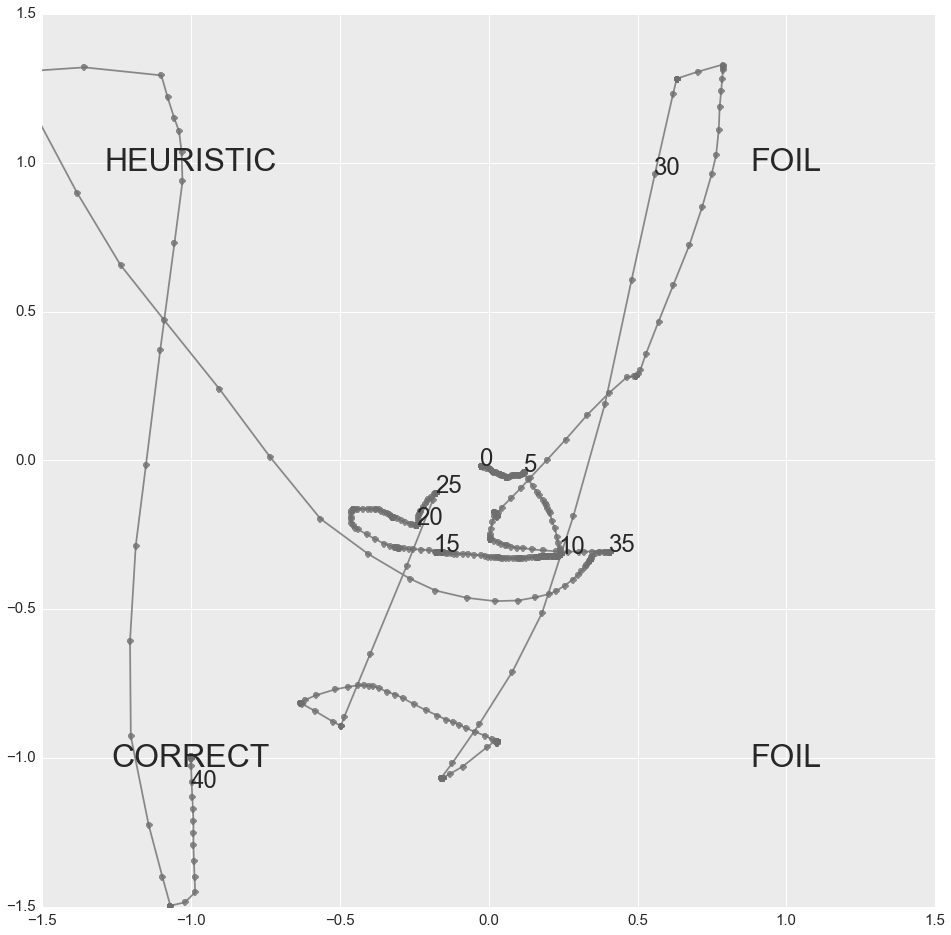
\includegraphics[width=\figurewidth]{imgs/exp6-typical-trajectory.png}
  \caption[A typical cursor trajectory from Experiment 6.]{
    \label{fig:exp6-typical-trajectory}
    A typical mouse cursor trajectory from the conflict condition. 
    Numerical values indicate the time elapsed in seconds. 
    Cursors meandered as participants generated their responses, 
    passing near the response options located in the corners of the display
  }
\end{figure}

In most previous mouse tracking research,
both in this thesis and in general
\citep[e.g.][]{Freeman2011d,Spivey2005},
the location of the cursor is recorded over a few seconds,
as participants move it from a starting position to 
a response option located in either top corner of the screen.
Almost invariably, this path follows either a single movement
(curved or otherwise) to a response,
or as has been more the case in this thesis,
a movement towards one response, that changes direction mid-flight.
In the current data, unfolding over up to 60 seconds, 
participants move and rest the cursor many times throughout a trial,
an average of 5.1 times, and a maximum of 30.
Thus, this data is in ways more similar to eye movement data.
A typical mouse cursor trajectory is shown in Figure~\ref{fig:exp6-typical-trajectory},
showing  a number of movements which pass near to several response options. 
In order to analyse participants' attraction to each response option over time,
the display was divided into quadrants
corresponding to each response option.
For the first 60 seconds of each trial, 
the mouse cursor positions at each 200 millisecond time slice
were coded according to which section of the screen they occupied, 
similar to fixation analyses of eye-tracking data.

Figure~\ref{fig:exp6-all} shows, for each response region, 
the proportion of trials in which the cursor is in that region, over time,
for both conflict and no-conflict problems. 
While the proportions at 60 seconds here 
largely reflect participants' ultimate responses, 
earlier proportions show how these preferences developed over time. 
Both correct responses to no-conflict problems and 
heuristic responses to conflict problems
were intuitively appealing, and participants 
began to move towards both options from before 5 seconds.
At approximately 10 seconds, participants also began to move towards
the correct response option on conflict problems,
and the accumulation of cursors in the region 
of the heuristic option under conflict slowed accordingly. 
The proportion of cursors in the region of these foil response options 
declined steadily in both conditions. 
Note that the proportions for the foil response options 
are averaged across the two foil options on conflict problems, 
and three options on no-conflict problems.

\begin{figure}[hp]
  \centering
  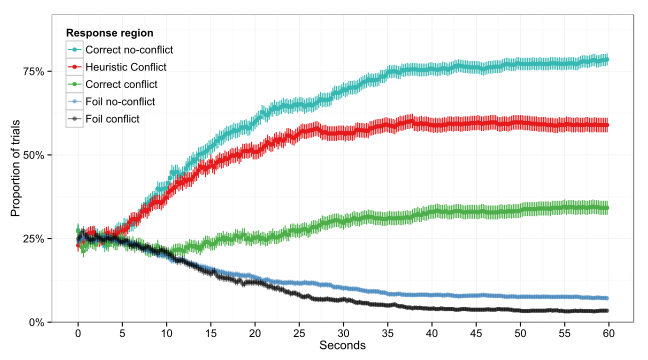
\includegraphics[width=\figurewidth]{imgs/exp6-all.pdf}
  \caption[Proportion of mouse cursors each region of the screen over time, Experiment 6.]{
    \label{fig:exp6-all}
    Proportion of mouse cursors in the region of the screen 
    corresponding to each response options, over time, 
    for conflict and no-conflict problems.    
  }
\end{figure}

\begin{figure}[bp]
  \centering
  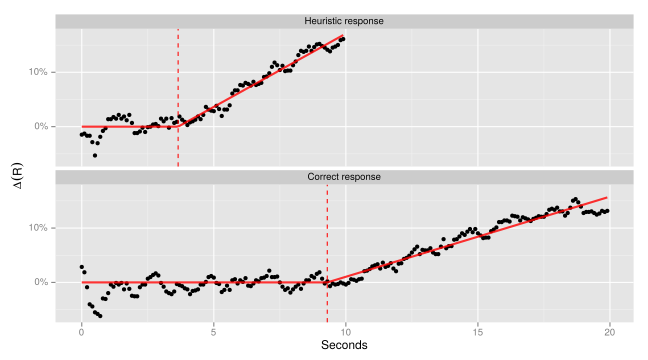
\includegraphics[width=\figurewidth]{imgs/exp6_changepoint.pdf}
  \caption[Change point analysis, Experiment 6.]{
    \label{fig:exp6_changepoint}
    Top: $\Delta (Heuristic)$, the difference between
    the probability of the cursor being in the region of the heuristic option
    and the probability of being in the region of a foil option.\\
    Bottom: $\Delta (Correct)$, the difference between
    the probability of being in the region of the correct option,
    and of being in the region of a foil option.
    Solid red lines show non-linear regression fits.
    Dashed vertical lines show change points,
    after which participants began to be drawn towards the option in question.
  }
\end{figure}

\subsubsection{Bayesian Change Point Analysis}

Inspecting Figure~\ref{fig:exp6-all},
participants are initially equally likely
to move toward each of the four response options
on conflict trials, doing so 25\% of the time.
This is the case until some time before 5 seconds,
at which point participants become more likely
to be in the region of the heuristic option
than the correct option, or either of the foils,
reflecting the point at which processes driving participants
towards the heuristic response exert their influence.
Similarly participants were equally likely to be
in the region of the correct option as the foils
until around 10 seconds,
and after this point more likely to be in the region of the correct option,
indicating that participants begin to be drawn towards the correct option
from this time.

Of course, visual inspection of these curves
is not a particularly accurate means of revealing
\emph{when} participants begin to be drawn towards each response option.
To formally estimate the times at which
participants began to move towards each response,
I calculated, across each 40 msec,
$\Delta (Heuristic)$: the difference between the average probability
of the cursor being in the region of the heuristic option
and the probability of being in the region of either foil option, as well as
$\Delta (Correct)$: the difference between the average probability
of being in the region of the correct option
and of being in the region of the foil option.
This yielded two series of values (Figure~\ref{fig:exp6_changepoint})
that were close to $0$ until participants
began to be drawn towards the response in question,
and increased over time after that point.

I modelled these series using a non-linear regression model
of the form

\begin{equation*}
  \Delta (R) =
  \begin{cases}%
    0          & \text{if}\ t\ <\ \tau_{R} \\
    \beta * (t-\tau_{R})  & \text{otherwise}%
  \end{cases}
\end{equation*}

where $t$ is the time in seconds,
$\tau_{R}$  is the point at which
participants begin to be drawn towards response $R$,
and $\beta$ is the slope of the regression line
after time $\tau_{R}$.

Modelling $\Delta (Heuristic)$, I analysed the first 10 seconds of each trial,
and set a uniform prior on the value of $\tau_{Heuristic}$ between 0 and 10 seconds
(i.e. that participants were equally likely to start being drawn
towards the heuristic response any time between 0 and 10 seconds into a trial).
Modelling $\Delta (Correct)$, I analysed the first 20 second,
and again set a uniform prior on $\tau_{Correct}$ between 0 and 20 seconds.
In both cases, I set an uninformative normal prior
with mean 0 and SD 1 on the slope, $\beta$.

Figure~\ref{fig:exp6_changepoint} shows the fitted regression models,
and Table~\ref{tbl:exp6_changepoint} shows the posterior estimates for the parameters.
The posteriors for the $\tau$ parameters represent
estimates of the point at which participants began to be drawn to each response.
The median posterior estimate for $\tau_{Heuristic}$ was
3.65 seconds (95\% credible interval [3.36, 3.93 seconds]),
and the estimate for $\tau_{Correct}$ was
9.30 seconds (95\% credible interval [8.86, 9.64 seconds]).
The $\beta$ parameters reflect how quickly
the proportion of participants in the region of each option increased after time $\tau$.
The estimate for $\beta_{Heuristic}$
(median 0.027, or a 2.7\% increase per second,
95\% credible interval [2.5\%, 2.9\%])
was almost twice as large as that for $\beta_{Correct}$
(median 0.015, or a 1.5\% increase per second,
95\% credible interval [1.4\%, 1.6\%]).
To summarise, participants began to be drawn towards
the heuristic option from 3.6 seconds,
and towards the correct option from 9.3 seconds.
After these onsets of attraction,
there was a greater increase in the proportion of trials
where the cursor was in the region of the heuristic option (2.7\% per second)
than in the proportion of trials
where it was in the region of the correct option (1.5\% per second).


\begin{table}
  \centering
  \caption[Bayesian change point analysis, Experiment 6.]{
    Posterior estimates from the change point analysis.
    Participants began to be drawn towards the heuristic option
    from 3.65 seconds, and the correct option from 9.30 seconds.
    \label{tbl:exp6_changepoint}
  }
  \begin{tabular}{lrrr}
    \toprule
    Parameter           & Median & 2.5\% & 97.5\%\\
    \midrule
    $\tau_{Heuristic}$  & 3.65  & 3.36 & 3.93\\
    $\tau_{Correct}$    & 9.30  & 8.86 & 9.64\\
    \midrule
    $\beta_{Heuristic}$ & 0.027  & 0.025 & 0.029\\
    $\beta_{Correct}$   & 0.015  & 0.014 & 0.016\\
    \bottomrule
  \end{tabular}
\end{table}



\subsubsection{Growth curve modelling}

\begin{figure}[ht]
  \centering
  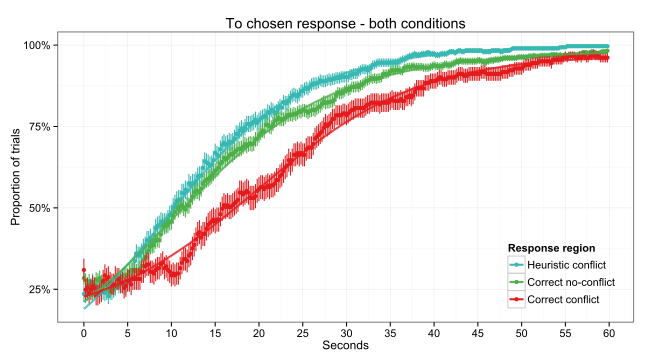
\includegraphics[width=\figurewidth]{imgs/exp6-all-to-chosen.pdf}
  \caption[Proportion of cursor in region of chosen response option, Experiment 6.]{
    \label{fig:exp6-all-to-chosen}
    Proportion of mouse cursors in the region of
    the response option which was ultimately selected on that trial.    
  }
\end{figure}

This time course data also allows us to
supplement the response time analyses reported above
by looking at the speed at which participants moved the mouse cursor to
the region of the response option they eventually did select.
Figure 4 shows this measure for correct responses to no-conflict problems,
and for both heuristic and correct responses to conflict problems.
The curve for each response region over time
was modelled using third-order polynomial logistic regression models
\citep[or growth curves; see][]{Mirman2014},
such that the log odds of the cursor being in that region were given as
$\alpha + \beta_1 t + \beta_2 t^2 + \beta_3 t^3$.
Natural polynomials were used,
meaning that the intercept corresponded to the log odds at 0 seconds,
the linear term to the simple change over time,
and the quadratic and cubic terms to higher-order 'wiggles' later in the time course.%
\footnote{
  One disadvantage of using these natural polynomial terms
  is that they are by definition correlated,
  and so the model suffers from mild multicollinearity,
  which leads to some loss of statistical power.
  However, as the alternative, orthogonal polynomial terms
  would be difficult to interpret individually,
  I believe this approach lends itself
  to a clearer description of the data.
  }

To test for a significant difference between two curves,
a null model, in which the  weights were the same for each curve,
was compared with a full model, in which there were different  weights for each curve.
Chi-squared tests were used to compare the deviance of each model,
with degrees of freedom corresponding to the number of  parameters added in the full model.
Note that $\alpha$, the intercept, was not allowed to vary between curves.
Finally, a random effect for the linear time term was included for each participant,
to allow for individual variability in
how quickly each participant moved towards a response in general.
Random effects on other terms, by participant, or by problem, were considered,
but led to convergence issues, and so only this term,
which was found to account for the most variance, was included.

Mirroring the response time analyses, and as predicted by all dual process accounts,
participant were faster to move towards
the heuristic response option when selecting it
than the correct option for conflict problems
($\chi^2$ = 4515.7, DF = 3, p < .0001),
with the curves differing significantly on the linear, quadratic, and cubic terms
(z's > 5, p's < .0001; see Figure~\ref{fig:exp6-all-to-chosen}).
Again consistent with the response time analyses,
and contrary to previous findings supportive of the intuitive logic model,
participants were faster to move towards the heuristic response on conflict problems
then to move towards the correct response on no-conflict problems
($\chi^2$, DF = 3, p < .0001).
This effect was mainly driven by a significant difference
on the linear term between the curves (z = 2.352, p = .0187).

Most dual process theories, including default-interventionist,
parallel-competitive, and intuitive logic accounts,
would predict that participants should be
drawn towards the heuristic option
on trials where they ultimately give the correct response.
In order to test for this attraction,
I compared the probability over time of
the cursor being in the region of the heuristic option
with the average probability of it being in the region of
either foil option on those trials (Figure~\ref{fig:exp6-correct-not-chosen}).
A higher probability of being in the region of the heuristic option
than the foils constitutes evidence of an attraction towards that heuristic response.
Visual inspection of Figure~\ref{fig:exp6-correct-not-chosen} shows that
this is the case from approximately 10 seconds onwards.
Again, third order polynomial regression models were fit to this data,
which showed that the difference between the curves was statistically significant
($\chi^2$ = 428.2, DF = 3, p < .0001),
with significant differences on the linear, quadratic, and cubic terms
(z's > 2.1, p's < .05).
Therefore, when selecting the correct response,
participants were more drawn to the heuristic option than to the foils,
as predicted both by default-interventionist
and parallel-competitive or intuitive logic accounts.

\begin{figure}[pt]
  \centering
  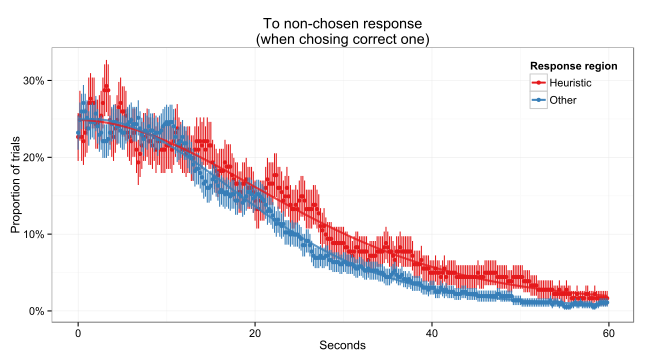
\includegraphics[width=\figurewidth]{imgs/exp6-correct-not-chosen.pdf}
  \caption[Proportion of cursor in region of other response options
  when correct response was given, Experiment 6.]{
    \label{fig:exp6-correct-not-chosen}
    Proportion of trials in the region of each option, over time,
    for trials in which the correct option was eventually chosen,
    for conflict problems.
    Error bars show standard error of measurement.
    Lines show fitted polynomial regression curves.
    Participants were more likely to be in the region of the heuristic response from around 10 seconds onwards.
  }
\end{figure}

\begin{figure}[pb]
  \centering
  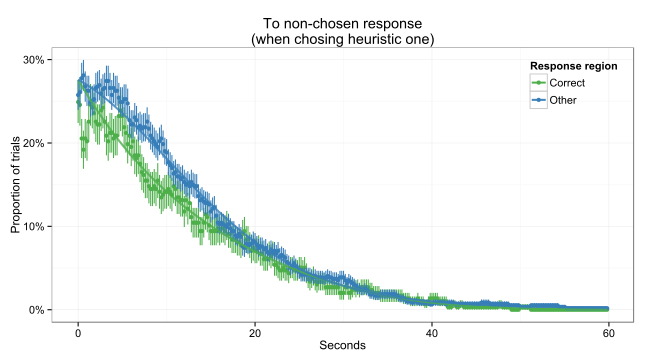
\includegraphics[width=\figurewidth]{imgs/exp6-heuristic-not-chosen.pdf}
  \caption[Proportion of cursor in region of other response options
  when heuristic response was given, Experiment 6.]{
    \label{fig:exp6-heuristic-not-chosen}
    Proportion of trials in the region of each option, over time,
    for trials in which the intuitive option was eventually chosen,
    for conflict problems.
    Participants were less or equally likely to be
    in the region of the correct option than a foil throughout.
  }
\end{figure}


A more interesting comparison is between
the attraction towards the correct response option,
and that towards the foil options,
on conflict trials where the heuristic response is given.
According to the default-interventionist account,
Type 2 processes have not become engaged at this point,
and so the correct response option should not be
any more attractive than the foil options.
According to the parallel-competitive account,
on the other hand, both Type 1 and Type 2 processes
should be engaged on such trials,
and so participants should be drawn towards
giving the response cued by Type 2 processes
(that is, the correct response).
Either result could be consistent with the intuitive logic theory,
depending on the mechanism by which conflict is actually detected.
If conflict detection occurs because
Type 1 processes simultaneously cue both the correct and heuristic responses,
then attraction towards the correct response option should be seen here.
Conversely, if conflict is detected
without Type 1 processes actually producing the correct response,
then the intuitive logic theory,
like the classic default-interventionist account,
would predict no attraction towards the correct response option here.
Of course, no conflict would be predicted by a selective theory.

Figure~\ref{fig:exp6-heuristic-not-chosen} shows that,
contrary to the prediction of the parallel-competitive
and intuitive logic accounts,
participants are not more likely to move towards the correct response option
than either of the foils before giving the heuristic response.
Participants were in fact less likely
to be in the region of the correct option than the foils.
The polynomial regression model showed that
the difference between the curves shown is again significant
($\chi^2$ = 208.0, DF = 3, p < .0001),
with significant differences between the curves on the
linear, quadratic, and cubic terms (z's > 9, p's < .0001).
This result indicates that the correct responses were on average
actually less attractive than the foils.
This is perhaps unsurprising,
given that part of the difficulty of the CRT
lies in the failure of intuition to support the correct response.

%% Finally, once again following previous tests of
%% the intuitive logic theory \citep[e.g.][]{Mevel2014},
%% I repeated the time course analyses reported above for both the
%% ``majority heuristic'' and ``minority heuristic'' participants.
%% The plots for these analyses are shown in Appendix~\ref{appendix:exp6_participants},
%% and reveal that my main findings hold for
%% both sets of participants.
%% \aside{This bit is tricky, especially after the reviews.
%%   Talk about by-item differences here?
%%   Eye balling them, there really is no difference for the bat and ball problems,
%%   but maybe I could test this?}
%% Appendix~\ref{appendix:exp6_items} shows the same analyses
%% plotted separately for each of the eight CRT problems.
%% Again, the results described broadly hold true across all items.
%% However, the bat-and-ball question
%% can be seen to differ slightly from the others
%% in some of the analyses here.
%% I explore this discrepancy in Appendix~\ref{appendix:exp6_items_model}.

\FloatBarrier


\subsection{Discussion}

In general, the results of this experiment
are consistent with Experiment 3,
but unlike in Experiment 3, I did not exclude any data
on the basis of the post-test results.
Participants' inferences were influenced by both
associative and structured knowledge.
Associative knowledge was indexed by the association ratio,
reflecting how strongly each participant rated
the association between the base and the correct species,
compared to the base and the foil.
This was a strong predictor of their inferences,
with participants more likely to project the property
to the correct species as its association with the base increased,
relative to the foil.
If participants only relied on associative knowledge, however,
they should give the correct response only 50\% of the time
when the association ratio favoured each response equally (ratio of $\frac{1}{1}$).
In reality, the fitted model predicted 72\% accuracy on such trials,
indicating that participants were also influenced
by structured taxonomic relationships.

Unlike Experiment 3, the current experiment revealed
that response times for correct responses were
marginally faster when the association ratio favoured the correct species
(i.e. when the associative and structured knowledge cued the same response).
There were, however, faster movement initiation times
for conflict trials in Experiment 3,
a finding that was not replicated here.
Of course, these two results are likely related:
initiation times are included in total response times,
and so faster initiation times under conflict in the previous experiment
may cancel out an overall effect on response time.
However, my analyses do not rest on these measures,
and so I will not attempt to interpret them further.

More interesting are the analyses of the cursor trajectories.
First, I found that initial cursor movements
were strongly predicted by associative knowledge,
and only marginally predicted by structured knowledge:
strength of association being equal,
participants are expected to move towards the correct species 62\% of the time.
After moving towards the correct species,
participants rarely
(20\% of the time when the species were equally associated)
changed direction to select the foil instead,
although they were more likely to do this
if the foil was more strongly associated than the correct species.
After initially moving towards the foil species, however,
participants were somewhat more likely to change direction:
they were predicted to do so 37\% of the time
when the association strengths were equal,
and more often when the correct species was more strongly associated.

From all of this, we can conclude three things.
First, associative knowledge predicts participants' movements
at every possible juncture, and unsurprisingly,
participants are more drawn towards a response option
when it is more strongly associated than the alternative.
Second, structured knowledge also plays a role at every juncture.
Participants were marginally more likely
to initially move towards the correct species
than would be expected based on associative knowledge alone,
and later, participants were in general more likely to change direction
to the correct species after initially moving towards the foil (37\%)
than to change to the foil species after
initially moving towards the correct one (20\%).
Third, once they started moving towards a response option,
participants in this experiment were unlikely to change direction.

Analysing the proportion of correct responses
where the cursor trajectory was classified as a reversal,
an unexpected trend emerged.
The data could be modelled using the association ratio as a predictor:
correct responses were more likely to involve
initial movements towards the foil
when the foil was more strongly associated than the correct species.
However, the data were slightly better fit by a model that
used the magnitude of this ratio
(how far it was from a ratio of $\frac{1}{1}$, in either direction),
resulting in the inverted U trend seen in Figure~\ref{fig:exp4_reversals}.

However, while this pattern was unexpected,
it can be understood in light of the transition probabilities, discussed above.
Participants were, first of all, more likely to
initially move towards the correct species
when the association ratio favoured this response.
Additionally, regardless of their initial movement,
participants were also more likely to ultimately select the correct species
when it was favoured by the association ratio.
Combined, these factors produce three kinds of trajectory.
When the association ratio strongly favoured the correct species,
participants moved straight towards that species, and selected it,
rarely moving to the foil at all,  and yielding few reversals.
When the ratio favoured the foil species,
participants who moved towards the foil usually ended up selecting it,
leaving few who moved to the foil before selecting the correct species.
When the ratio did not favour either species, however,
some participants  moved towards the foil initially,
and some of these changed their minds,
yielding a higher number of reversal trajectories.

Finally, the time course trends here are consistent with those found in Experiment 3.
As the association ratio becomes stronger in favour of the correct species,
participants became more likely to ultimately select this species,
but there were no striking changes in the trends leading up to these responses.
Additionally, consistent with the analysis of the transition probabilities,
even when associative and structured knowledge conflicted strongly,
there was no indication that participants were
first driven by associative knowledge,
and then by structured knowledge.
This is again consistent with the trends seen for Experiment 3.




\section{General Discussion}


In these two experiments
participants completed versions of the inductive triad task
where they were asked to generalise a property from a base category
to one or other response category.
They could rely either on conceptual knowledge,
and so generalise the property to the category that
belonged to the same category as the base,
or on perceptual cues,
and generalise to the category that looked like the base.
In both experiments, I manipulated whether the cues agreed or disagreed,
so that on conflict trials perceptual cues would lead participants
to select the foil response option rather than the
conceptually-related one.
On these conflict trials, participants were
more likely to select the foil category.
Furthermore, they were more likely to make
fast initial mouse movements towards the foil,
which they often overrode to select the correct category instead.
These results are consistent with \citegap{Bright2014a}{'s} hybrid theory of induction.

I also raised the question of how perceptual cues
and conceptual knowledge might interact during induction.
One option was that participants
selectively relied on perceptual cues \emph{or} conceptual knowledge.
The alternative was that participants were
initially driven by perceptual cues,
but sometimes overrode theses cues when they realised them to be inappropriate,
and relied on conceptual knowledge instead.

The results showed that participants,
although usually initially moving towards the perceptually-cued foil,
sometimes moved directly towards the conceptually-cued option,
with these movements generally taking longer to initiate
than those towards the foil.
There are two possible explanations for such trials.
It may be that participants simply draw on conceptual knowledge here,
a process which takes longer, and then act on it.
Alternatively, participants on these trials
may have first processed the perceptual cues,
but inhibited them and replaced them with their conceptual knowledge
before initiating their cursor movement.
It is not clear at present how these possibilities could be disentangled,
and so for the time being this particular issue remains an open question.

In Experiment 2, I manipulated the kinds of properties participants reasoned about:
either specific properties, that were saliently related
to the distinction between the two categories,
or generic properties, that were not.
This manipulation mainly affected what participants did
on trials where they initially moved towards a perceptually-cued foil option.
Participants reasoning about specific properties were
significantly more likely to override their initial movement
and select the correct option instead
than those reasoning about generic properties.
The manipulation did not make participants any less likely
to initially move towards the foil option,
and its influence on the time course data
emerged relatively late in reasoning (see Figure~\ref{fig:exp2_foil_side_timecourse}).
It also had no influence on control trials,
where participants almost invariably selected the correct option.
Therefore, it would appear that this manipulation
mainly served to make participants more likely
to inhibit their perceptually-driven responses
on trials in which they were initially driven towards giving them.
This is consistent with much previous work,
both using the current paradigm \citep{Gelman2013c}
and other inductive tasks \citep{Heit1994,Ross1999},
indicating that the kind of information people draw on in inductive reasoning
is contingent on the nature of the properties to be projected.
A future question raised by this result concerns
whether this manipulation serves to make
participants more likely to inhibit perceptual cues,
or if it makes certain structured knowledge
easier to retrieve by cuing or priming it.

The purpose of these experiments
was to investigate adults' inductive reasoning,
and the results are consistent with \citegap{Bright2014a}{'s} hybrid account.
Specifically, they suggest that induction cannot be explained entirely
by either accounts based on unstructured associative knowledge
such as (perceptual or representational) similarity
\citep[i.e.][]{Sloman1993,Rogers2004,Sloutsky2004,Fisher2015}
or by purely structured, conceptual knowledge
\citep[i.e.][]{Osherson1990,Griffiths2009,Kemp2009,Gelman1986}.
Instead, both kinds of information appear to influence adults' reasoning,
with simple perceptual similarity drawn on earlier in the process,
and perhaps serving as a default.
However, these results also have implications for theories of children's reasoning.
As discussed in Chapter 1, and earlier in the current chapter,
a number of experiments have claimed to show that
young children's inferences are either
driven by conceptual knowledge
\citep{Gelman2013c,Rhodes2009,Gelman2007a,Gelman1986},
or that they are driven by perceptual similarity
\citep{Sloutsky2008,Sloutsky2007,Sloutsky2004a}.
These previous experiments \citep[i.e.][]{Gelman1986,Sloutsky2007,Gelman2013c},
however, have focused on a binary question:
do children draw on perceptual cues, \emph{or} on conceptual knowledge during reasoning?
Therefore, these experiments only presented participants with conflict trials,
and their responses were classed as either
consistent with reliance on perceptual similarity,
consistent with reliance on conceptual knowledge,
or not significantly different from chance in either direction.
As discussed in Chapter 1,
an experimental control condition, of the type used here,
where both cues agree, makes it possible to discover
not only which cue dominates when both conflict,
but also whether the neglected cue,
perceptual similarity in this case,
has any influence at all.

Therefore, these results with adults suggest a new interpretation
of the developmental data:
if both perceptual similarity and conceptual knowledge influence adults' reasoning,
they likely both also play a role in children's inferences.
This perspective may make sense of
apparently contradictory results in the developmental literature,
where children seem to draw on conceptual knowledge
in some scenarios but not others.
It is likely that these studies differ
in terms of the factors which make participants
more or less likely to inhibit initially influential perceptual cues.
Thus, while children may have access to both perceptual cues
and information about conceptual knowledge across all of these experiments,
they are more likely to inhibit the former in favour of the latter
when categories differ at a high, ontological level,
when entities are more easily categorised,
or when the properties under consideration are
conceptually related to the distinction between the categories
\citep{Gelman2013c}.
In short, the current results suggest that
developmental researchers should be less concerned
about \emph{whether} children rely on similarity or on conceptual knowledge,
and instead ask \emph{when} do children rely on either form of information.



% \aside{ This is where Newall 20 questions with nature bit comes in! }







% Having shown that perceptual and conceptual knowledge
% are activated during induction,
% our next question is how to these representations
% interact during the reasoning process.
% \aside{I need to look at trajectories when the wrong response was chosen.}
% Unlike a number of mouse tracking studies
% that found graded, continuous attraction towards both responses \citep[i.e.][]{Spivey2005},
% we found that participants moved directly towards one or other response,
% and on many trials moved initially towards one, before changing direction mid-flight.
% Earlier trajectories were more likely to be directed
% towards the perceptually-cued response option
% while later movements moved towards the conceptually-related option.
% This is consistent with the idea that only one representation
% can exist in working memory at a time.










\begin{appendices}
  %% \setcounter{secnumdepth}{0}
  \appendixpage
  \graphicspath{{./../Appendices/}}
  
  \chapter{Stimuli from Experiment 1}\label{appendix:exp1_stimuli}
    %% http://tex.stackexchange.com/a/88939/60964
  % \centering
  %%   \hspace*{-2cm} \begin{tabular}{rcccc}
  %%   \toprule
  %%   Set & Base species                     & Correct option                & Conflict foil                 & Control foil \\
  %%   \midrule
  %%   1   & \smallpic{imgs/bird}             & \smallpic{imgs/flamingo}      & \smallpic{imgs/bat}           & \smallpic{imgs/fox}          \\
  %%   2   & \smallpic{imgs/dandelions}       & \smallpic{imgs/roses}         & \smallpic{imgs/coral_flower}  & \smallpic{imgs/coral_brain}  \\
  %%   3   & \smallpic{imgs/bug_leafy}        & \smallpic{imgs/bug_ladybird}  & \smallpic{imgs/plant_leaf}    & \smallpic{imgs/tree_winter}  \\
  %%   4   & \smallpic{imgs/hedgehog}         & \smallpic{imgs/dog}           & \smallpic{imgs/pinecone}      & \smallpic{imgs/sycamore}     \\
  %%   5   & \smallpic{imgs/dino_triceratops} & \smallpic{imgs/dino_sauropod} & \smallpic{imgs/rhino}         & \smallpic{imgs/cat}          \\
  %%   \bottomrule
  %% \end{tabular}\hspace*{-2cm}
  \vspace*{-2cm}\begin{longtable}{rcccc}
    \caption[]{ Stimulus images used in Experiment 1.} \label{} \\
    
    \toprule
    Set & Base species                     & Correct option                & Conflict foil                 & Control foil \\
    \midrule
    \endfirsthead

    \toprule
    Set & Base species                     & Correct option                & Conflict foil                 & Control foil \\
    \midrule
    \endhead

    %% \hline \multicolumn{3}{|r|}{{Continued on next page}} \\ \hline
    \bottomrule
    \endfoot
    
    \bottomrule
    \bottomrule
    \endlastfoot

    1   & \smallpic{imgs/exp1/bird}             & \smallpic{imgs/exp1/flamingo}      & \smallpic{imgs/exp1/bat}           & \smallpic{imgs/exp1/fox}          \\
    2   & \smallpic{imgs/exp1/dandelions}       & \smallpic{imgs/exp1/roses}         & \smallpic{imgs/exp1/coral_flower}  & \smallpic{imgs/exp1/coral_brain}  \\
    3   & \smallpic{imgs/exp1/bug_leafy}        & \smallpic{imgs/exp1/bug_ladybird}  & \smallpic{imgs/exp1/plant_leaf}    & \smallpic{imgs/exp1/tree_winter}  \\
    4   & \smallpic{imgs/exp1/hedgehog}         & \smallpic{imgs/exp1/dog}           & \smallpic{imgs/exp1/pinecone}      & \smallpic{imgs/exp1/sycamore}     \\
    5   & \smallpic{imgs/exp1/dino_triceratops} & \smallpic{imgs/exp1/dino_sauropod} & \smallpic{imgs/exp1/rhino}         & \smallpic{imgs/exp1/cat}          \\
    6   & \smallpic{imgs/exp1/tuna}             & \smallpic{imgs/exp1/fish_yellow}   & \smallpic{imgs/exp1/dolphin}       & \smallpic{imgs/exp1/badger}       \\
    7   & \smallpic{imgs/exp1/lime}             & \smallpic{imgs/exp1/strawberry}    & \smallpic{imgs/exp1/fish_green}    & \smallpic{imgs/exp1/mackerel}     \\
    8   & \smallpic{imgs/exp1/duck}             & \smallpic{imgs/exp1/eagle}         & \smallpic{imgs/exp1/platypus}      & \smallpic{imgs/exp1/kangaroo}     \\
    9   & \smallpic{imgs/exp1/leopard}          & \smallpic{imgs/exp1/deer}          & \smallpic{imgs/exp1/leopard_gecko} & \smallpic{imgs/exp1/gecko}        \\
    10  & \smallpic{imgs/exp1/fish_stripey}     & \smallpic{imgs/exp1/goldfish}      & \smallpic{imgs/exp1/zebra}         & \smallpic{imgs/exp1/horse}       \\
    
\end{longtable}\vspace*{-2cm}
  %% \caption[]{}



  \chapter{Post test scores for stimuli used in Experiment 1} \label{appendix:exp1_posttest}
  \begin{table}[h!]
  \centering
  \begin{tabular}{rrr}
    \toprule
    Base                  &  Correct response  (Accuracy)   & Conflict foil       (Accuracy)   \\
    \midrule                                                                                     
    Bird                   & Flamingo           (92\%)  & Bat                  (85\%) \\
    Dandelions             & Roses              (98\%)  & Coral (flower-like)  (82\%) \\
    Insect (leaf-like)     & Insect (Ladybird)  (93\%)  & Plant (leafy)        (100\%)\\
    Hedgehog               & Dog                (87\%)  & Pinecone             (100\%)\\
    Dinosaur (Triceratops) & Dinosaur (Sauropod) (91\%)  & Rhino                (68\%) \\
    Tuna                   & Fish (yellow)      (95\%)  & Dolphin              (71\%) \\
    Lime                   & Strawberry         (100\%) & Fish (green)         (100\%)\\
    Duck                   & Eagle              (92\%)  & Platypus             (73\%) \\
    Leopard                & Deer               (95\%)  & Leopard Gecko        (97\%) \\
    Fish (stripey)         & Goldfish           (100\%) & Zebra                (95\%) \\
    \bottomrule
  \end{tabular}
  \caption[]{
    Accuracy on the post-test for stimuli pairs used in Experiment 1.
    Scores greater than 67.8\% are significant at the p < .01 level.
    }
\end{table}



  \chapter{Properties used in Experiment 2}\label{appendix:exp2_properties}
  
Properties were presented in the form ``This one X. Who else do you think X''.

\textbf{Properties specific to Flurps (animals)}

\begin{itemize} 
  \singlespacing
    \item This one breathes. 
    \item This one can have babies. 
    \item This one has a heart inside. 
    \item This one has a mummy. 
    \item This one has bones inside. 
    \item This one needs water. 
    \item This one can climb trees. 
    \item This one tries to stay warm. 
\end{itemize}

\textbf{Properties specific to Floobits (robots)}
\begin{itemize}
\singlespacing
    \item This one can be turned off. 
    \item This one can break. 
    \item This one has batteries inside. 
    \item This one has wires inside. 
    \item This one was made by people. 
    \item This one was sold in a store. 
    \item This one is cold touch. 
    \item This one doesn't sleep. 
\end{itemize}

\textbf{Generic properties}
\begin{itemize}
\singlespacing
    \item This one can make a zevy sound. 
    \item This one has a very sticky toma. 
    \item This one has zimmer inside. 
    \item This one is used for derriping. 
    \item This one needs tiddles to make it move. 
    \item This one uses danner. 
    \item This one can help yippets. 
    \item This one goes outside in the winter. 
    \item This one has a part inside called a cece. 
    \item This one has blickets inside of it. 
    \item This one has grumpets that make it strong. 
    \item This one is good for kertling. 
    \item This one is found on farms. 
    \item This one can be very old. 
    \item This one feels yinty. 
    \item This one lacks ombelots. 
\end{itemize}



\end{appendices}


\bibliography{../references}
\addcontentsline{toc}{chapter}{References}



\end{document}
